\documentclass[12pt,a4paper]{article}
\usepackage[utf8]{inputenc}    % Encodage UTF-8
\usepackage[T1]{fontenc}       % Caractères français corrects
\usepackage{subcaption}
\usepackage{float}
\usepackage[french]{babel}     % Langue française
\usepackage{geometry}          % Marges
\usepackage{hyperref}          % Liens et sommaire cliquable
\usepackage{biblatex}
\usepackage{graphicx}          % Citations et bibliographie
\addbibresource{bibliographie.bib}

\geometry{margin=2.5cm}

\title{
  \textbf{\LARGE Rapport de Stage / Mi-parcours} \\[1ex]
  \large Effet de l'alaitude sur le développement des enfants vivant au Pérou
}
\author{Lancelot RAVIER\\Master 1 Statistiques et Sciences de Données}
\date{Année universitaire 2024--2025}


\begin{document}

% Page de garde
\maketitle
\begin{center}

\includegraphics[width=12cm]{logo.png} \\[2ex]
\end{center}
\thispagestyle{empty}
\newpage

% Sommaire
\tableofcontents
\newpage

% Introduction
\section*{Introduction}
\addcontentsline{toc}{section}{Introduction}
Le projet \textbf{Expedition 5300}, initié au Pérou, s'inscrit dans une démarche scientifique visant à comprendre les effets de la très haute altitude sur la santé des péruviens habitant dans des villes de très haute altitude (< 3000m). Mené par une équipe franco-péruvienne de chercheurs de tous horizons, cette expédition combine analyses médicales, physiologiques et biologiques dans le but d'explorer les mecanismes d'adaptation du corps humain à l'hypoxie chronique dans les zones habitées les plus hautes du monde, dans lesquelles les populations portent une grande valeur aux questions de santé et sont donc très ouvertes aux analyses médicales.

Dans ce contexte, mon stage s'est concentré sur l'étude de l'impact de l'altitude sur la santé des enfants vivant au Pérou et sur les différentes techniques de détection de l'anémie/polyglobulie, à travers une analyse comparative menée dans quatre villes situées à des altitudes croissantes : Lima (150m), Cusco (3400m), Juliaca (3800m) et La Rinconada (5300m, ville la plus haute du monde), chez une population d’enfants âgés de 0 à 3 ans et de 8 à 12 ans, exposés à l’environnement local de façon continue depuis la période prénatale, sans changement de lieu de vie depuis la grossesse. L'objectif principal est de mieux comprendre comment l'exposition prolongée à l'hypoxie influence le développement physiologique des enfants, notament en ce qui concerne l'oxygénation, la croissance, l'hématologie (composition du sang) et les marqueurs d'adaptation. Le sang est composé de globules rouges transportant l'oxygène ($\sim 45\%$), de plasma ($\sim 55\%$) et de globules blancs ($\sim <1\%$). Deux phénomènes opposés mais liés sont au cœur de cette étude : l'anémie et la polyglobulie. L'anémie se caractérise par une concentration en hémoglobine (protéine attachée aux globules rouges permettant de transporter l'oxygène dans le sang) insuffisante dans le sang, ce qui peut limiter le transport de l’oxygène et affecter la croissance et le développement des enfants. À l’inverse, la polyglobulie correspond à une concentration excessive d’hémoglobine, souvent en réponse à l’hypoxie chronique, mais qui peut augmenter la viscosité du sang et engendrer des risques cardiovasculaires. La définition clinique de ces états peut varier avec l’altitude, ce qui justifie une analyse spécifique et comparative dans ce contexte.

Ainsi, ce travail s'inscrit à la fois dans une perspective de santé publique locale (en analysant la pertinence des techniques de détection d'anomalies du sang et en identifiant les facteurs de risques liés à l'altitude) et dans une ambition scientifique plus large visant à compléter la littérature scientifique avec des analyses portées sur l'adaptation à l'altitude d'une population précise, celle des péruviens.

% Partie 1
\section{Présentation du laboratoire HP2}
Le laboratoire Hypoxie Physiopathologie Performance (HP2) est une unité mixte de recherche attachée à l'Université Grenoble Alpes, à l'INSERM et au CHU Grenoble Alpes. Il est situé à l'Hôpital sud de Grenoble, en déménagement vers l'UGA.
Le laboratoire HP2 s'intéresse aux effets de l'hypoxie, du sommeil et de l'activité physique sur la santé, en particulier dans les domaines de cardiologie, pneumologie et métabolisme humain. Les projets de recherche menés par les équipes du laboratoire visent à mieux comprendre comment ces facteurs peuvent influencer le développement et l'évolution des maladies chroniques, avec une attention portée sur les mecanismes physiopathologiques, à l'identification de biomarqueurs et à la médecine de précision.
L'approche du laboratoire est pluridisciplinaire, combinant recherche fondamentale, recherche clinique et études de populations. Le laboratoire HP2 mène en parallèle certains projets originaux en conditions extrêmes au travers d'expéditions scientifiques comme "Expédition 5300" dans les Andes péruviennes, afin d'étudier l'hypoxie d'altitude chez ces populations.

\section{Présentation des données}

La base de données utilisée pour les analyse est composée de 632 enfants (nés et vivant dans leur ville de naissance et pré-natale), distribués de la manière suivante selon l'âge et la ville :

\begin{table}[h!]
\centering
\begin{tabular}{lcccc}
\hline
\textbf{Tranche d'âge} & \textbf{Lima} & \textbf{Cusco} & \textbf{Juliaca} & \textbf{La Rinconada} \\
\hline
0--3 ans   & 49  & 114 & 48  & 58 \\
8--12 ans  & 83  & 59  & 125 & 96 \\
\hline
\end{tabular}
\caption{Répartition du nombre d'enfants par ville et tranche d'âge (ordre croissant d'altitude : 150m < 3400m < 3800m < 5300m)}
\end{table}

Les variables utilisés dans le cadre des premiers résultats sont les suivantes :

\begin{itemize}
  \item \textbf{[Hb]} : concentration d’hémoglobine dans le sang (g/dL)
  \item \textbf{Hb\_mass} : masse totale d’hémoglobine (g ou g/kg pdc.)
  \item \textbf{Anemie/Polyglobulie (OMS2011)} : variable indicatrice du résultat du diagnostic après avoir corrigé [Hb] selon les critères OMS2011
  \item \textbf{Anemie/Polyglobulie (OMS2024)} : variable indicatrice du résultat du diagnostic après avoir corrigé [Hb] selon les critères OMS2024
  \item \textbf{Anemie (-1SD, -2SD)} : diagnostic mathématique de l'anémie en selectionnant toutes les observations à -1 ou -2 écarts-types selon la moyenne de [Hb]
  \item \textbf{Anemie (+1SD, +2SD)} : diagnostic mathématique de la polyglobulie en selectionnant toutes les observations à +1 ou +2 écarts-types selon la moyenne de [Hb]
\end{itemize}

% Partie 2
\section{Missions réalisées}

\subsubsection{Analyse des différences entre méthodes de détection d'anémie}

L'anémie et la polyglobulie sont détéctées par l'analyse de la concentration d'hémoglobine dans le sang. Cependant, en altitude, l'hypoxie entraine naturellement une élévation des taux d'hémoglobine comme mecanisme d'adaptation. En 2011, l'OMS proposait des seuils ajustés en fonction de paliers fixes d'altitude appliqués uniformément à toutes les populations. En 2024, l'OMS a actualisé ses recommandations en introduisant une approche continue et contextuelle en tenant en compte à la fois de l'altitude, de l'âge, du sexe et des adaptations physiologiques spécifiques des différentes populations constituant les données.
Ainsi, le premier objectif de ce stage était de comparer (concordances, discordances, différences inter-villes) les deux techniques de détection entre-elles, ainsi que de comparer chacune d'elles à des techniques de détection mathématiques ($\pm 1$ ou $2$ SD) avec comme finalité l'apport de preuve aux médecins péruviens de la pertinence de la technique ajustée de 2024 de l'OMS dans la détection de l'anémie chez les populations péruviennes.

% Partie 3
\section{Bilan}
\subsection{Premiers résultats}

\subsubsection{Différences intra-villes dans la détection de l'anémie}

Pour analyser les différences intra-villes entre méthodes de détection de l’anémie, nous avons produit des barplots de prévalence par ville et méthode, séparément pour les 0–3 ans et les 8–12 ans. Les données ont été restructurées au format long, avec une variable binaire indiquant la présence d’anémie. Des tests globaux (Chi² ou Fisher selon les effectifs) ont été réalisés, ville par ville, pour détecter une hétérogénéité entre méthodes. Lorsque significatifs, des comparaisons deux-à-deux ont été menées à l’aide des mêmes tests. Les p-values ont été transformées en annotations de significativité classiques et affichées sur les graphiques.

\begin{figure}[H]
    \centering

    \begin{subfigure}{0.48\textwidth}
        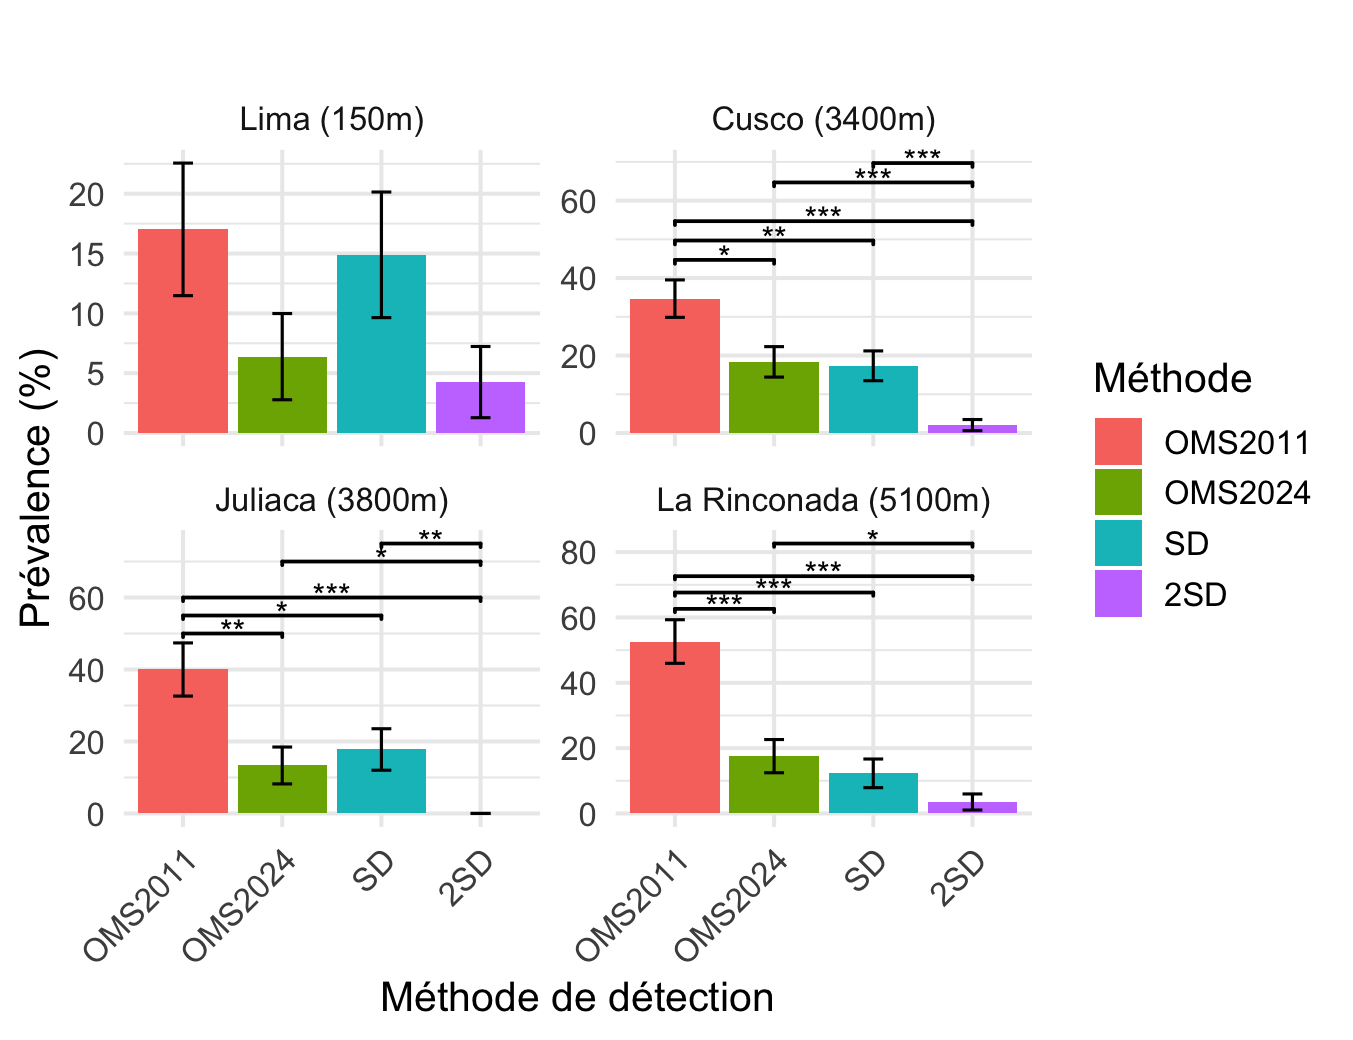
\includegraphics[width=\linewidth]{Rplot.png}
        \caption{Figure 1.1 - Prévalence par ville (0–3 ans)}
        \label{fig:pre03}
    \end{subfigure}
    \hfill
    \begin{subfigure}{0.48\textwidth}
        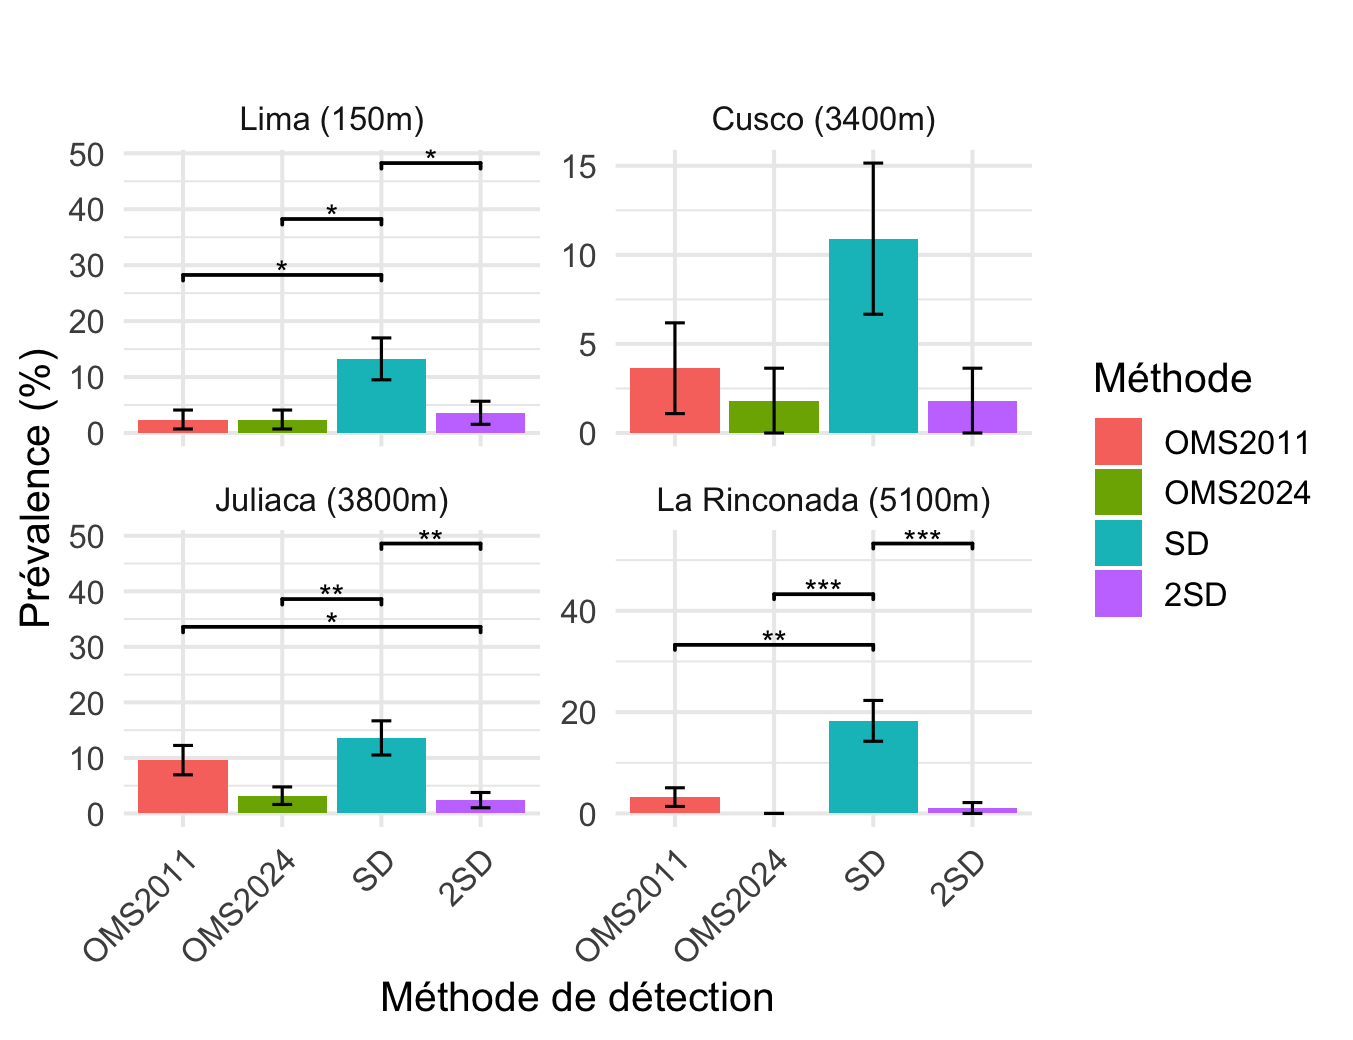
\includegraphics[width=\linewidth]{Rplot12yo.png}
        \caption{Figure 1.2 - Prévalence par ville (8–12 ans)}
        \label{fig:pre812}
    \end{subfigure}

    \caption{Prévalence de chaque méthode de détection de l'anémie, chez les enfants de 0–3 ans (gauche) et 8–12 ans (droite). (*** p < 0.001, ** p < 0.01, * p < 0.05)}
    \label{fig:pre}
\end{figure}

Ainsi, selon les graphiques ci-dessus :
Chez les enfants de 0-3 ans (Figure 1.1), la méthode OMS 2011 donne des prévalences élevées dans toutes les villes, particulièrement en haute altitude (Cusco, Juliaca, La Rinconada), où elles dépassent parfois les 50\%. La révision proposée par OMS2024 réduit significativement ces prévalences, en particulier en altitude. En plaine (Lima), les prévalences sont modérées avec OMS2011 et SD, plus faibles avec OMS2024 et très basses avec 2SD. A l'inverse à La Rinconada, la méthode OMS2011 détecte une prévalence très élevée, tandis que les autres méthodes ne détectent que peu d'anémiques.
Chez les enfants de 8-12 ans (Figure 1.2), les profils sont différents. En plaine (Lima), toutes les méthodes donnent des prévalences faibles, sauf SD, dont l'écart est significatif avec les autres méthodes (attendu car méthode mathématique). Cet effet est aussi remarqué en haute altitude où il est plus marqué.

D'après ces deux graphiques, on observe donc que les nouvelles diréctives de l'OMS de 2024 induisent une réduction significative du nombre d'enfants détectés comme anémiques en comparaison aux seuils de 2011. La différence entre les 0-3 ans et les 8-12 ans peut être due au fait qu'avec l'âge, les enfants s'acclimatent et donc leur taux d'hémoglobine augmente naturellement.


\subsubsection{Concordances entre les méthodes}

Afin de quantifier le degré d'accord entre les différentes méthodes de détection de l'anémie, des coefficients de Kappa de Cohen ont été calculés deux-à-deux pour chaque paire de méthodes. Cette analyse permet d'évaluer dans quelle mesure les méthodes classent les mêmes individus comme anémiques ou non, indépendamment de la prévalence globale. Chaque ligne de la matrice de kappa correspond à la valeur du Kappa de Cohen entre deux méthodes, calculés à partir de leur concordances sur l'ensemble des enfants d'une tranche d'age donnée. Les résultats ont été représentés sous forme de matrices symétriques colorées. Chaque case contient la valeur numérique du Kappa. Le dégradé de couleur va du bleu (faible concordance, voire non significative si p<0), au rouge (forte concordance).

\begin{figure}[H]
    \centering

    \begin{subfigure}{0.48\textwidth}
        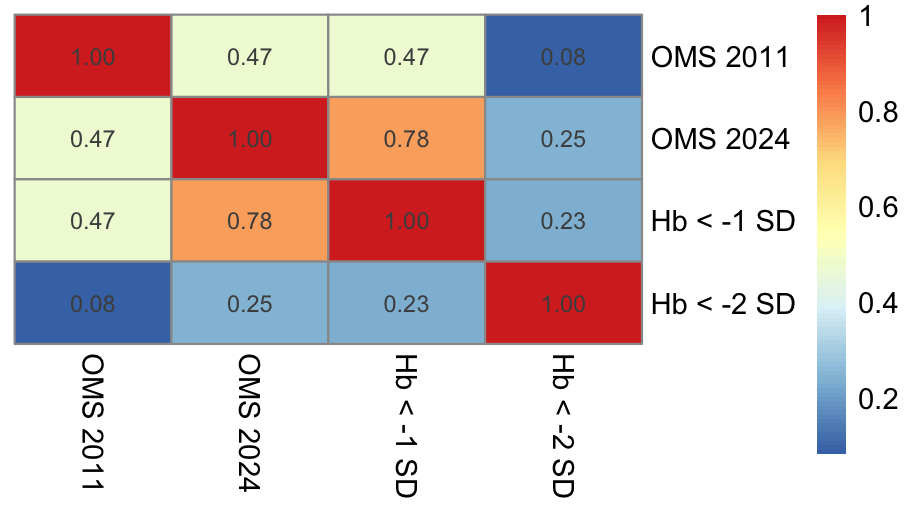
\includegraphics[width=\linewidth]{kappa3.png}
        \caption{Concordance entre méthodes (0–3 ans)}
        \label{fig:kappa_0_3}
    \end{subfigure}
    \hfill
    \begin{subfigure}{0.48\textwidth}
        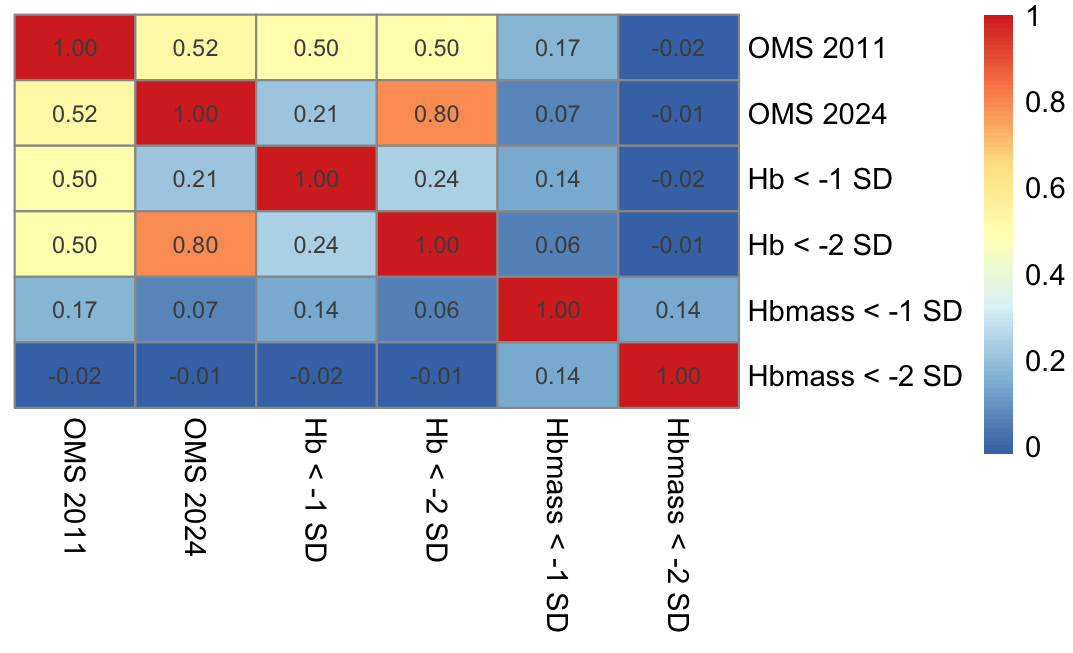
\includegraphics[width=\linewidth]{kappa12.png}
        \caption{Concordance entre méthodes (8–12 ans)}
        \label{fig:kappa_8_12}
    \end{subfigure}

    \caption{Coefficients de Kappa de Cohen mesurant l’accord entre différentes définitions de l’anémie, chez les enfants de 0–3 ans (gauche) et 8–12 ans (droite).}
    \label{fig:kappa_matrices}
\end{figure}

Ainsi, selon les deux figures ci-dessus :

Chez les 0-3ans, OMS2011 montre une concordance modérée (k = 0.47) avec OMS2024. De plus, OMS2024 a une concordance largement supérieure à OMS2011 pour les seuils mathématiques (SD, 2SD).

Chez les 8-12 ans, la concordance entre OMS2011 et OMS2024 est plus élevée (k = 0.52). La méthode OMS2024 est très concordante avec la méthode conservatrice 2SD, et la concordance entre OMS2011 et SD/2SD est modérée et égale. En revanche, les méthodes basées sur Hbmass présentent des valeurs k très faibles voir négatives, avec toutes les autres méthodes, révélant une quasi-absence d'accord.

Ainsi, chez les enfants de 0-3ans, les méthodes OMS2024 et SD apparaissent proches en terme de classification individuelle. Cependant, chez les 8-12 ans, les méthodes OMS et SD sur l'[Hb] brésentent des accords faibles à modérés (sauf pour OMS2024 et 2SD), mais les approches basées sur la masse d'[Hb] s'en détachent nettement. Ce résultat suggère que la méthode OMS2024 concorde en moyenne mieux que la méthode OMS2011 avec SD et 2SD, et que les méthodes physiologiques détectent un tout autre profil d'enfants anémiques.

\subsubsection{Discordances entre les méthodes}

Afin de tester les divergences de classification entre les méthodes OMS et mathématiques, une analyse croisée bivariée a été réalisée sur les données. Un test de McNemar a été appliqué aux tables de contingences 2x2 croisant les deux diagnostics. Ce test permet de détécter toute asymétrie significative entre les cas discordants. En fonction du nombre de discordances, un test exact de McNemar a été appliqué (si <25 discordants) ou un test de McNemar classique (chi-carré).

Les neuf graphiques suivants comparent les classifications d’anémie selon les seuils de l’OMS (2011 et 2024) à des méthodes basées sur des écarts-types de l’Hb ou de l’Hbmass. Un test de McNemar (ou exact selon les effectifs) évalue les discordances.

Le graphique 1 (OMS 2011 vs OMS 2024) révèle une forte discordance (40\,\% reclassés), $p \sim 0$. Le graphique 2 (OMS 2011 vs -1SD) montre une asymétrie importante (63\,\% vs 10\,\%), $p \sim 0.039$. Le graphique 3 (OMS 2011 vs -1SD\_Hbmass) indique un déséquilibre modéré, $p \sim 0.004$. Le graphique 4 (OMS 2011 vs -2SD) présente un désaccord très marqué (84\,\%), $p \sim 0$. Le graphique 5 (OMS 2011 vs -2SD\_Hbmass) montre également une discordance significative (6\,\%), $p \sim 0.003$.

Le graphique 6 (OMS 2024 vs -1SD) révèle une forte discordance (42\,\%), $p \sim 0$, tandis que le graphique 7 (OMS 2024 vs -1SD\_Hbmass) montre une discordance plus faible (6\,\%), bien que significative, $p \sim 0$. Le graphique 8 (OMS 2024 vs -2SD) indique une discordance inverse importante (86\,\%), $p \sim 0$. Enfin, le graphique 9 (OMS 2024 vs -2SD\_Hbmass) présente une quasi-absence de discordance (2\,\%), avec un test non significatif ($p \sim 0.508$).

Ces résultats suggèrent que les seuils OMS 2024 sont mieux alignés sur les définitions physiologiques strictes, en particulier celles fondées sur la masse d’hémoglobine.

% Conclusion
\section*{Conclusion et analyses en cours}
\addcontentsline{toc}{section}{Conclusion}
Les premiers résultats des analyses de méthodes de détection de l'anémie confirme l’importance cruciale du choix de la méthode de détection dans l’estimation de la prévalence, en particulier en contexte d’altitude et selon l’âge des enfants. Les anciennes directives de l’OMS de 2011 apparaissent systématiquement plus sensibles, au point de probablement surestimer l’anémie chez les enfants vivant en altitude. Cette tendance est atténuée par les nouvelles recommandations OMS2024, qui conduisent à une réduction significative du nombre de cas détectés.

Les comparaisons avec des méthodes mathématiques (SD, 2SD) ou physiologiques (Hbmass/kg) mettent en évidence des discordances marquées, mais aussi certaines convergences intéressantes. En particulier, OMS2024 montre une meilleure concordance avec des méthodes plus strictes ou physiologiquement fondées, comme 2S\_Hbmass, suggérant une calibration plus pertinente des seuils de diagnostic.

Plusieurs autres analyses sont en cours, dans lesquelles nous allons essayer d'analyser les différences entre l'hémoglobine et la masse d'hémoglobine comme mesure du transport d'oxygène. Aussi, nous avons reçu des données de tests neurologiques et catégories socio-professionnelles, et nous sommes dans l'attente des mesures relative à la supplémentation en fer des enfants vivants en altitude, de laquelle nous allons pouvoir analyser de manière approfondie l'effet de la classification comme anémique de nombreux enfants sur leur supplémentation en fer et les effets sur l'hemoglobine de cette supplémentation en fer, en particulier pour les enfants qui ne sont plus détectés comme anémiques avec la nouvelle directive de 2024.

% Bibliographie
\printbibliography

\end{document}
